
\documentclass[12pt]{article}
%% Language and font encodings
\usepackage[portuguese]{babel}
\usepackage[utf8x]{inputenc}
\usepackage[T1]{fontenc}

%% Sets page size and margins
\usepackage[a4paper,top=2.5cm,bottom=2.5cm,left=3cm,right=3cm,marginparwidth=1.75cm]{geometry}

%% Useful packages
\usepackage{amsmath}
\usepackage{graphicx}
\usepackage[colorinlistoftodos]{todonotes}
\usepackage[colorlinks=true, allcolors=blue]{hyperref}

\title{Revisão sobre o Modelo Gravitacional do Comércio}
\author{Gustavo Alovisi}

\begin{document}
\maketitle

\begin{abstract}
Este trabalho tem como objetivo realizar uma revisão do Modelo Gravitacional do Comércio, criado por Jan Timbergen em 1962. O autor propõe um modelo para determinar o padrão do comércio internacional e como ele é construído. O modelo possui um bom ajuste empírico e facilidade de estimação e manuseio. Será feita uma revisão do modelo e sua evolução na história econômica. Será também apresentado o método para estimar o Modelo Gravitacional do comércio, para dados em painel de diversos países e dados em cross-section para a análise do volume do comércio, importação e exportação entre o Brasil e diversos países. 
\end{abstract}

\section{Introdução}

Jan Timbergen, antes de seguir sua carreira na economia e ganhar um nobel em 1969, graduou-se em física pela Universidade de Leiden. Sua análise da dinâmica do comércio internacional baseou-se no Modelo de Gravitação Universal de Isaac Newton, que mensura a força de atração de dois objetos, baseado em suas massas, distância e força gravitacional. O resultado de que na ausência de barreiras ao comércio, um determinado país tende a ter como principal parceiro comercial outro país de PIB próximo e distância relativamente pequena mostrou ter um bom ajuste empírico observável até os dias de hoje. Desde a publicação de seu estudo até os dias atuais, diversos métodos para a estimação do modelo gravitacional surgiram, assim como fundamentações teóricas baseadas em teorias do Comércio Internacional como uma tentativa de explicar a robustez do ajuste empírico do modelo. 

\section{O Modelo Gravitacional}

\subsection{Gravitação Universal e Comércio Internacional}

A Lei da Gravitação Universal postulada por Isaac Newton no século XVII define a força de atração entre dois corpos como proporcional entre o produto de suas massas e inversamente proporcional à sua distância ao quadrado. A Lei é representada pela seguinte equação: \[F_g =\frac{M_1 * M_2}{D_{12} ^2}\] sendo Fg a atração entre os dois corpos, M1 a massa do primeiro corpo, M2 a massa do segundo corpo e D² o quadrado da distância entre eles. Já o modelo básico de Timbergen para o comércio entre dois países pode ser descrito pela equação: \[E_{ij} = a_o * Y_i ^{a_1} * Y_j ^ {a_2} * D_{ij} ^ {a_3}\] sendo $E_{ij}$ a exportação do país i para o país j, $Y_i$ o PNB do país i, $Y_j$ o PNB do país j, $D_{12}$ a distância entre eles e os demais termos constantes a serem estimadas. A analogia entre o modelo do Comércio Internacional e da Gravitação Universal é explicado da seguinte forma: a exportação ($E_{ij}$) é uma variável explicada que depende das variáveis independentes do lado direito da equação assim como a Força gravitacional ($F_g$) na Lei newtoniana. Originalmente o tamanho da exportações dependia de três fatores: \begin{enumerate}
\item O tamanho da economia do país exportador ($Y_i$). É entendido por Tim como o PNB do país e busca mensurar a capacidade de Oferta do mesmo.  
\item O tamanho da economia do país importador ($Y_j$). É entendido por Tim como o PNB do país e busca mensurar a capacidade de Demanda do mesmo.
\item A distância entre ambos ($D_{ij}$). Busca mensurar os diversos custos relacionados ao comércio entre os países, como os custos de transporte, transação, conhecimento de mercado e informação.
\end{enumerate} 

\subsection{O ajuste do modelo básico}
	Ao realizar a estimação, era esperado que os parâmetros $a_0, a_1 e a_2$ fossem números positivos para refletir a hipótese de que quanto maior a economia dos países maior a exportação (comércio) entre eles \cite{fabio1}. Em relação ao termo $a_3$, era esperado que sua estimação retornasse um valor negativo para refletir a hipótese da distância entre os países ser inversamente proporcional ao comércio entre eles. 
Para testar o ajuste de seu modelo, Timbergen utilizou-se de métodos econométricos e testou seu modelo em um conjunto de 18 países com seus dados para o ano de 1958 (cross-section). Foi também realizado novos testes em sua regressão, como a adição de variáveis dummy para determinados vínculos entre países. A regressão linear utilizada para a estimação do modelo básico de Timbergen foi a seguinte: \[ln E_{ij} = \beta_0 + \beta_1 * ln Y_i + \beta_2 * ln Y_j + \beta_3 * ln D_{ij} + \epsilon\]  
	O resultado dos testes de Timbergen foi positivo, com coeficientes $a_0, a_1, a_2$ positivos, $a_3$ negativo, coeficiente de determinação satisfatório e bons resultados nas adições de variáveis dummy. O modelo, portanto, mostrou um ajuste empírico robusto e despertou a atenção de pesquisadores e tomadores de decisão, dado seu grau de ajustamento empírico, relativa simplicidade e facilidade de manuseio e modificação, apesar de não estar teoricamente bem fundamentado.  

\subsection{A evolução do modelo gravitacional}
	A partir da proposta de Timbergen e da exposição de seus bons resultados, diversos estudos buscaram fundamentar teoricamente o modelo ou ainda expandir seu poder de previsão e ajustamento. Linneman (Linneman, 1966) por exemplo, afirmou que o modelo seria uma forma reduzida de uma análise de equilíbrio parcial, com quatro equações de oferta de exportação e 4 equações de demanda por importação. Leamer e Sters levantaram três hipóteses: Uma baseada na física, a segunda reduzindo equações de demanda exógena e variáveis de oferta e a terceira em um modelo probabilístico. Nenhuma delas obteve grande sucesso. (ANDERSON, 1979)
    \linebreak Uma das justificativas teóricas mais difundidas para a utilização do modelo gravitacional remete ao modelo de comércio desenvolvido por Krugman (1980), que considera que os consumidores buscam variedade ao consumir. Sendo assim, haveria diferenciação do produto entre as firmas monopolisticamente competitivas, não somente entre os países, Assim, um país com maior produção teria maior capacidade de satisfazer os anseios dos consumidores ao ofertar uma ampla gama de produtos. Soma-se a isso o fato de as economias com grande produção tenderem a gastar muito com importações, haja vista sua alta renda. Desta forma, o comércio entre duas economias seria tanto maior, quanto maiores fossem seus PIBs. Para justificar a influência da distância no modelo, os principais aspectos destacados são que a distância aumenta os custos de transporte, e, além disso, a comunicação e o fluxo de informações devido a diferenças culturais e idiomáticas aumentam os custos de informação acerca de leis, sistema tributário e outras regulamentações do país de destino, o que levaria países mais distantes a comerciar menos. 
    \linebreak Krugman, em 1980, Krugman e Helpman 1985 e Berstrand, em 1985 e 1989, mostraram, em algum nível, que a equação da gravidade podia derivar de modelos com bens diferentes; que produtos diferenciados poderiam surgir por países de origem, por economia de escala, por tecnologia, por abundância de certos recursos naturais. A razão para a diferenciação ou especialização pode ser diferente, mas todas elas gerariam forças de gravidade. \cite{sohn} (SOHN, 2005) \linebreak Atualmente, o modelo possui diversas fundamentações baseadas em diferentes teorias do comércio internacional, como o modelo de proporção de fatores, o modelo Heckshler-Ohlin e o modelo de competição monopolística. Deardoff (DEARDOFF, 1998) argumenta que o modelo gravitacional do comércio pode não comprovar as teorias do comércio internacional, mas que ele é muito eficaz em representar um 'fato da vida'. A partir de diversos estudos e ajustamentos para o modelo em relação a estas teorias, o modelo é em geral bem aceito pela comunidade acadêmica. \linebreak Hoje em dia, as maiores críticas em relação ao modelo não dizem respeito a sua fundamentação teórica, mas sim em relação aos métodos econométricos mais eficientes para estimar o modelo. 

\begin{figure}[h]
\centering
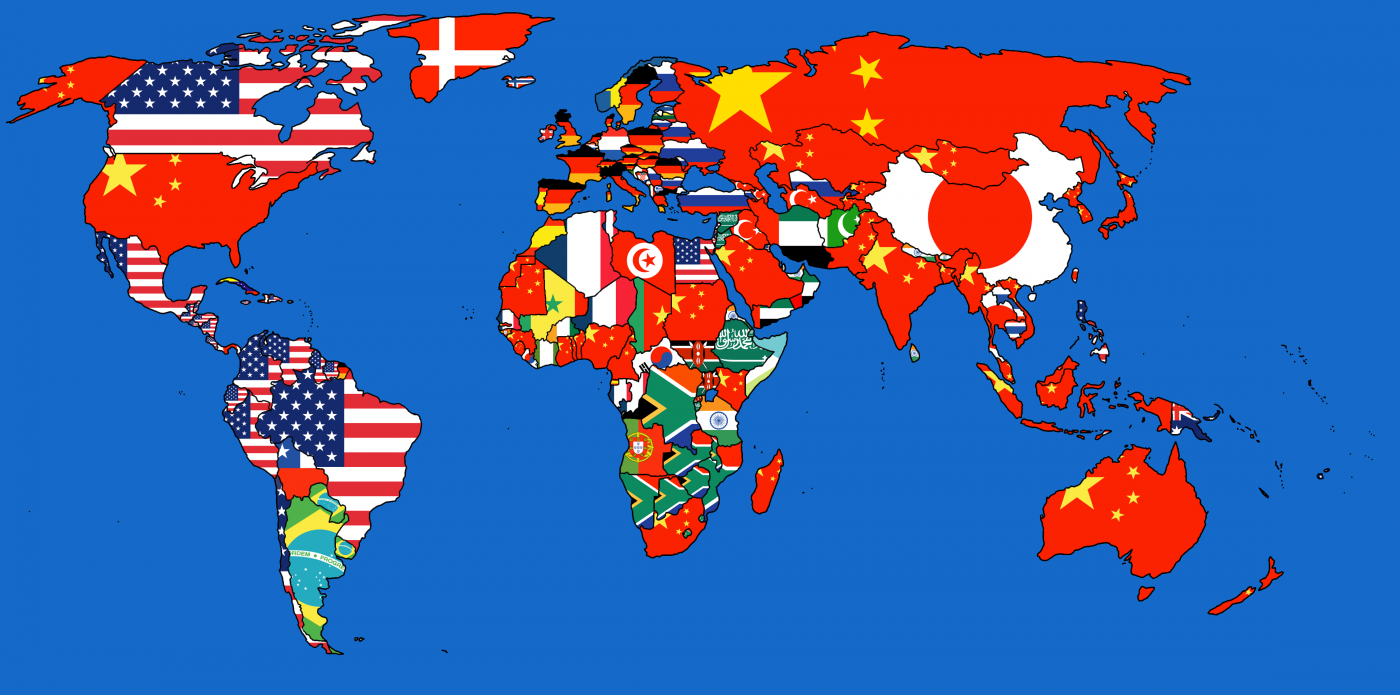
\includegraphics[width=0.6\textwidth]{mapa_importsdesenho.png}
\caption{\label{fig:imports}Imagem representativa do modelo de gravitação do comércio internacional. A imagem mostra, para o ano de 2012 o principal parceiro comercial dos países mundiais. É possível observar como a distância entre países e a semelhança do PIB relacionam-se com o estabelecimento de importantes parceiros comerciais.}
\end{figure}

\subsection{O modelo gravitacional expandido: dados em painel}
Um dos melhores resultados em relação ao modelo gravitacional do comércio é a sua facilidade de adaptação em relação a diferentes variáveis e acontecimentos em nível macroeconômico.  O modelo proposto em sua forma básica é utilizado para medir o volume esperado de comércio entre nações, porém, o próprio Timbergen já apresentava possibilidades de adaptação do modelo, com o uso de variáveis dummy.  \linebreak Atualmente, variáveis explanatórias como população, PIB per capita ou área do país são utilizadas em estimações da regressão, assim como variáveis de controle que buscam diferenciar características específicas de um país, como ambos países possuírem a mesma língua, cultura, fronteira ou bloco comercial. A utilização destas diversas variáveis pode, se desejado, transformar o objeto de análise do modelo que é a relação comercial entre os países para uma análise de políticas comerciais e como elas afetam o fluxo do comércio estabelecido. \linebreak Estudos em relação ao impacto de políticas específicas realizados incluem, por exemplo, os efeitos do protecionismo, da abertura comercial, a análise de formação de blocos e regiões comerciais e o comércio dentro e fora do país, chamado efeito-fronteira. Estudos alternativos incluem também a aplicação para a explicação de fluxos migratórios e fluxos de capital, e fluxos de investimento direto externo. \linebreak O modelo do comércio expandido pode ser estimado em relação a dados em painel ou cross-section. Dados em painel representam dados multi-dimensionais de diversos indivíduos ou características ao longo do tempo. Já dados em cross-section representam dados de países ou indivíduos para apenas um ponto no tempo. 



\begin{table}[h]
\centering
\begin{tabular}{l l l l}
Pessoa & Ano & Sexo & Renda\\\hline
1 & 2001 & 1 & 1000 \\
1 & 2002 & 1 & 1005 \\
1 & 2003 & 1 & 1003 \\
2 & 2001 & 0 & 4000 \\
2 & 2002 & 0 & 4000 \\
2 & 2003 & 0 & 5000 \\
\end{tabular}
\caption{\label{tab:widgets}Dados em painel. Podemos ver os dados de duas pessoas para diferentes períodos de tempo.}
\end{table}
    
\begin{table}[h]
\centering
\begin{tabular}{l l l}
Pessoa  & Sexo & Renda\\\hline
1  & 1 & 1000 \\
2  & 0 & 2000 \\
3  & 0 & 4000 \\
4  & 1 & 5000 \\
5  & 1 & 1300 \\
6  & 1 & 4320 \\
\end{tabular}
\caption{\label{tab:crosssec}Dados em cross-section. Exibe dados de diferentes pessoas para o mesmo período de tempo.}
\end{table}

\begin{figure}[h]
\centering
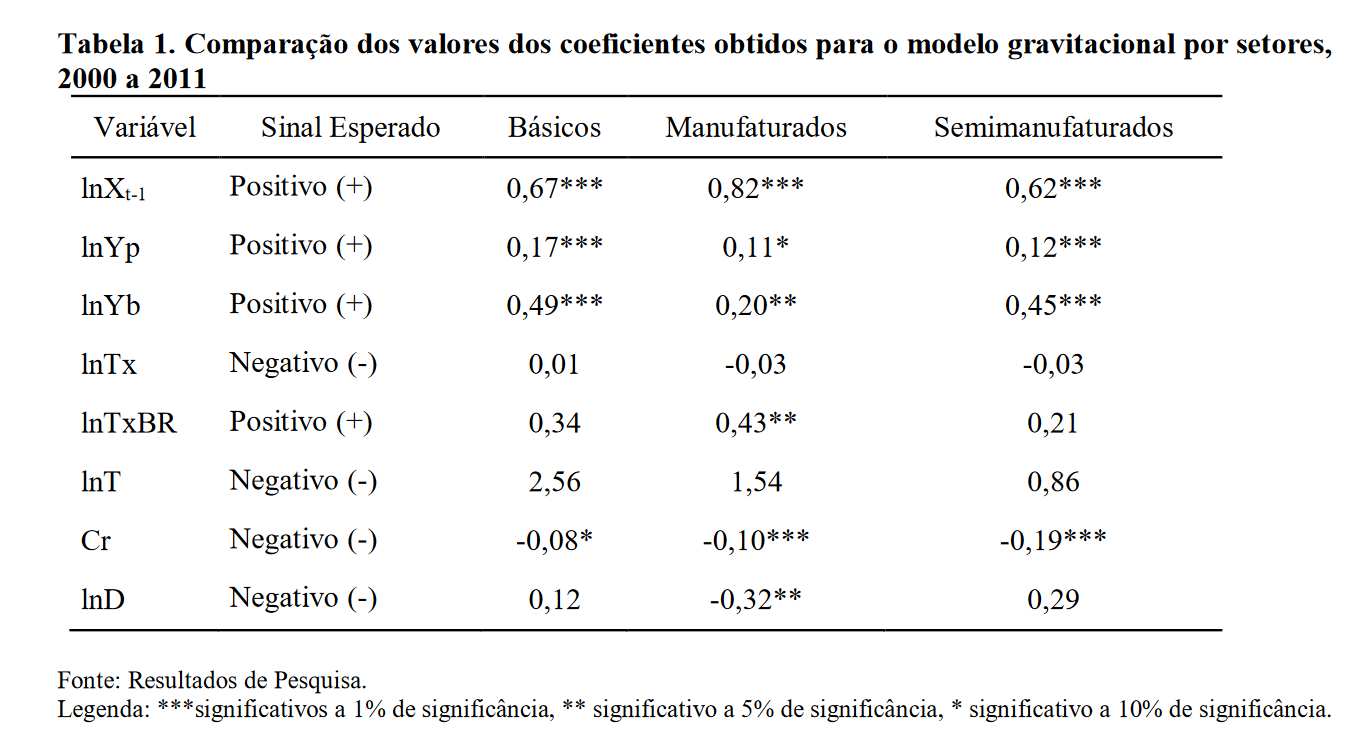
\includegraphics[width=1\textwidth]{panel1.png}
\caption{\label{fig:panel1}Estimação dos coeficientes do modelo expandido para dados em painel}
\end{figure}

O modelo expandido da gravitação do comércio para dados em painel que variam no tempo pode ser descrito pela seguinte equação: \[ln m_{ijt} = \alpha_t + \alpha_{it} + \beta_1 ln Y_{it} + \beta_2 ln Y_{jt} + \sum{\beta_{rtak} RTA_{ijt} + \beta_{td} TD_{ijt}} + \alpha X_{ijt} + \epsilon\]. \linebreak Onde, 
\begin{itemize}
\item $m_{ijt}$ representa o comércio bilateral entre os países i e j no tempo t;
\item $Y_{wt}$ é o PIB nominal dos países i e j no tempo t;
\item $RTA_{ijt}$ é uma dummy que assume valor= 1 se os países i e j pertencem a um mesmo acordo comercial regional k;
\item $TD_{ijt}$ é a dummy que assume valor =1 se pelo menos um dos dois países é um membro do acordo regional k; 
\item $\alpha_{ij}$ é o efeito fixo ao longo do tempo;
\item $\alpha_t$ o efeito fixo de cada ano;
\item $X_{ijt}$ é um vetor de outros pares de características dos países
\item $\epsilon_t$ é o erro composto no tempo t
\end{itemize}

De acordo com Eichengreen et al. (1995), os coeficientes das principais variáveis do modelo gravitacional assumem, como resultados esperados:

\begin{itemize}
\item Positivo para o coeficiente do PIB per capita do país importador e da elasticidade-renda da demanda do país importador;
\item Positivo para o coeficiente do PIB total do país importador por refletir o efeito de tamanho;
\item Geralmente positivo para o coeficiente do PIB per capita do país exportador, pois este deve ser pensado como uma medida de nível de produção do país  exportador, o que estaria relacionado com a relação capital trabalho deste país;
\item Positivo para o coeficiente do PIB total do país exportador, pois este sugere o quanto vasta pode sera variedade de produtos que o país tem a oferecer;
\item Negativo para o coeficiente da variável distância, visto que seu efeito deve ser considerado que quanto maior distância, maior o custo relativo dos produtos,implicando como inibidor do comércio.
\end{itemize}


Uma análise utilizando o modelo gravitacional do comércio com dados em painel pode ser encontrada em \cite{elizama1}. O autor faz uso do modelo gravitacional do comércio para estimar o Potencial do Comércio Internacional do Brasil para o período de 2000 a 2011. A estimativa dos coeficientes do modelo pode ser encontrada na Figura 2. 




\subsection{O modelo gravitacional do comércio expandido: dados em cross-section}
O modelo expandido para dados em cross-section pode ser descrito segundo a equação: \[ln m_i = \beta_0 + \beta_1 ln Y_i + \beta_2 ln Y_j + \beta_3 ln D_{ij} + \beta_4 Mar_i \beta_5 Port_i + \beta_6 AC_i + \epsilon\] Onde, 
\begin{itemize}
\item $ln m_i$ representa o comércio total entre o pais i e outros paises, ou ainda pode ser substituido para Importação ou Exportação 
\item $\beta_0$ é uma constante de participação comercial
\item $\beta_1 ln Y_i$ é o PIB do país i 
\item $\beta_2 ln Y_j$ é o PIB do país j 
\item $\beta_3 ln D_{ij}$ é a distância entre os países i e j
\item $\beta_4 Mar_i$ é uma variável dummy para a presença ou não de saída par ao mar do país i
\item $\beta_5 Port_i$ é uma variável dummy para a presença ou não de portos em i 
\item $\beta_6 AC_i$ é uma variável dummy para a presença ou não de acordos comerciais preferenciais. 
\item $\epsilon$ é o termo de erro da regressão
\end{itemize}


Uma estimava para os fluxos de comércio internacional utilizando dados em cross-section (dados em apenas um período no tempo) para o Brasil pode ser encontrado em \cite{beatriz1}, na qual a autora estima, utilizando o modelo em cross-section, os fluxos de comércio esperado entre Brasil e outros países para o ano de 2012. 
A figura 3 apresenta a estimação dos coeficientes do modelo do comércio expandido, para a regressão entre o Brasil e diversos outros países do mundo, com a variável dependente sendo (i) as exportações (ii) as importações (iii) o comércio total. Podemos notar que de fato diversos coeficientes são significantes a 1 porcento. 
A figura 4 apresenta uma avaliação do modelo aplicado às exportações entre Brasil e os outros países do mundo. São apresentadas as exportações reais para o ano de 2012 e as exportações previstas conforme o modelo. 
Países pequenos como Santa Lúcia aparecem como outliers devido a acordos comerciais únicos entre os países, principalmente de combustíveis fósseis. Hong King, Cingapura e Países Baixos também aparecem com um grande volume de comércio, principalmente pela presença de portos que escoam suas importações para o resto das determinadas regiões. Os EUA aparecem, ao contrário, como uma superestimação de atividade comercial prevista. No geral, porém, o modelo parece ter um bom ajustamento com valores de exportação prevista que não diferem muito das exportações de fato realizadas. 

\begin{figure}[h]
\centering
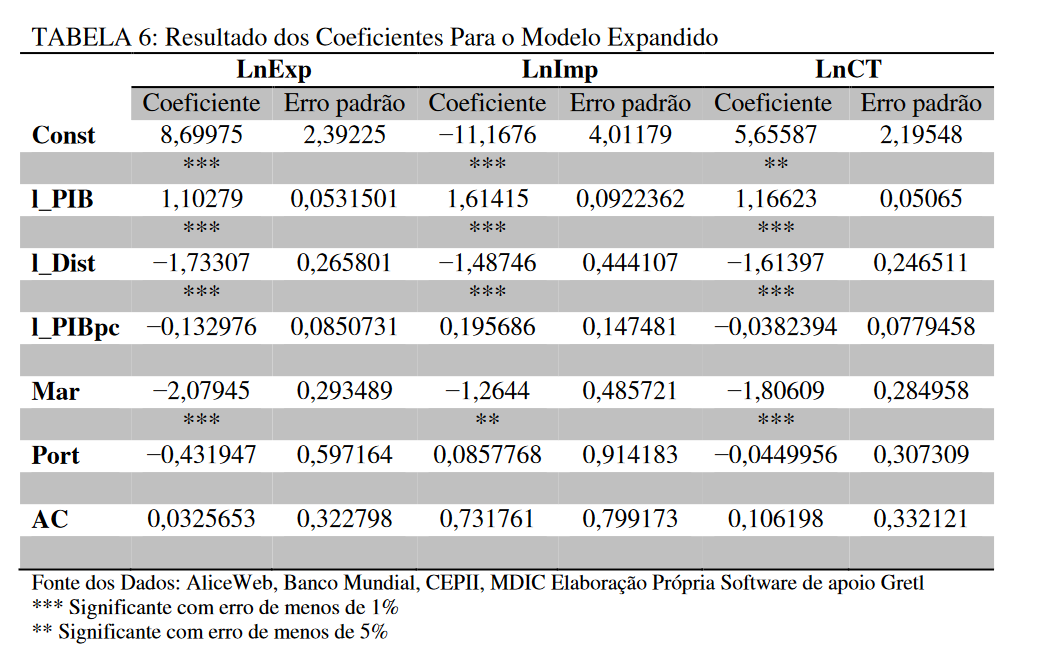
\includegraphics[width=1\textwidth]{crosssec.png}
\caption{\label{fig:coefscrossec}Estimação dos coeficientes do modelo expandido para dados da economia brasileira e outros países do mundo, em cross-section}

\end{figure}

\begin{figure}[h]
\centering
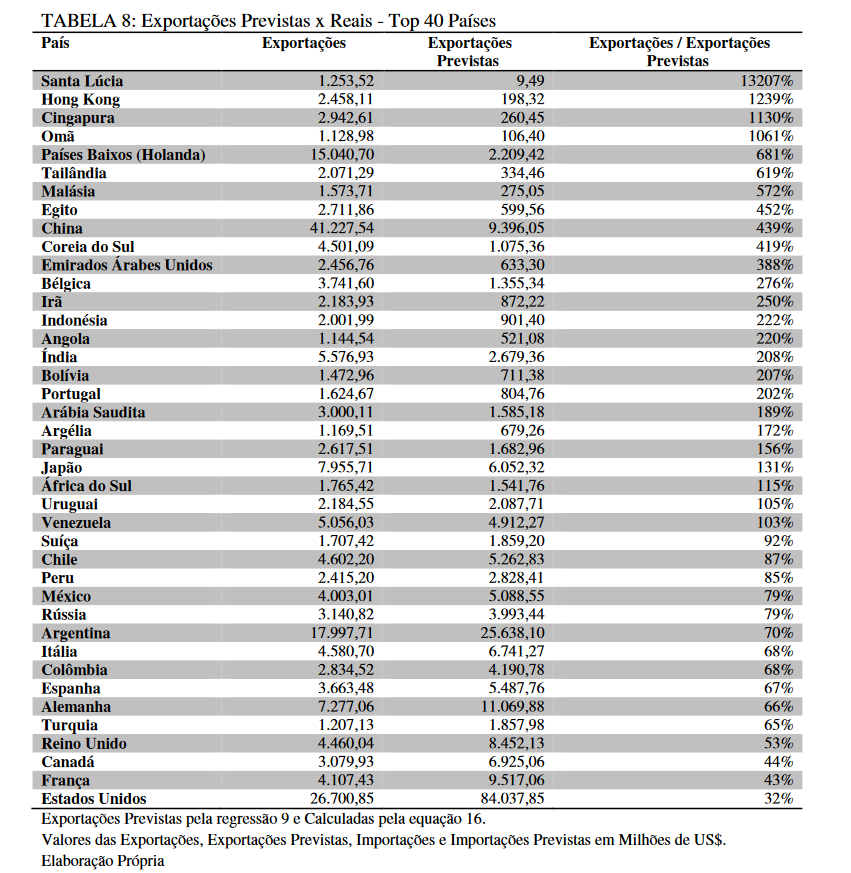
\includegraphics[width=1\textwidth]{crossec2.png}
\caption{\label{fig:crossec2}Avaliação do modelo de gravitação do comércio em relação as exportações brasileiras para diversos países em 2012.}
\end{figure}

\section{Conclusão}
A partir da análise histórica e empírica do modelo de gravitação universal do comércio internacional, podemos perceber sua relevância empírica para a análise de fluxos esperados de comércio entre países, bem como análise de políticas comerciais e acontecimentos macroeconômicos. Ao permitir um fácil manuseio para a estimação das variáveis e adição de diversas outras variáveis de controle, bem como uma robustez em seus ajustamentos, o modelo gravitacional do comércio se torna uma importante ferramenta empírica. 


\bibliographystyle{alpha}
\bibliography{sample}

\end{document}